
\section {Search for Dijet Resonance}

\subsection {The Signal: Dijet Resonance}


\begin{figure}[hbt]
  \begin{center}
     \includegraphics[width=0.45\textwidth]{Figures/shape_500GeV.pdf}
      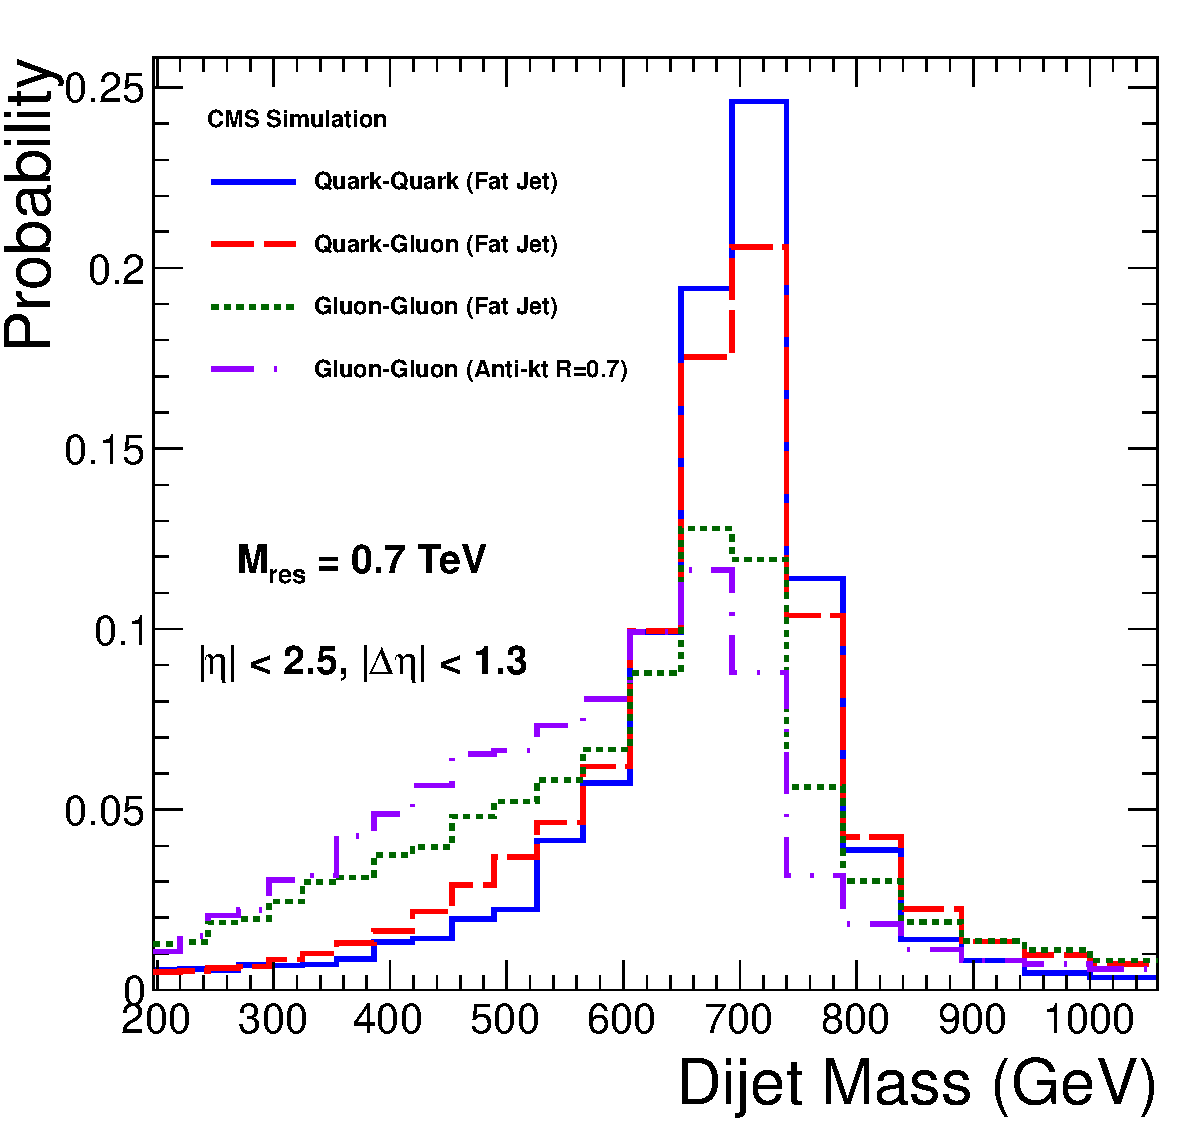
\includegraphics[width=0.45\textwidth]{Figures/shape_700GeV.pdf}
       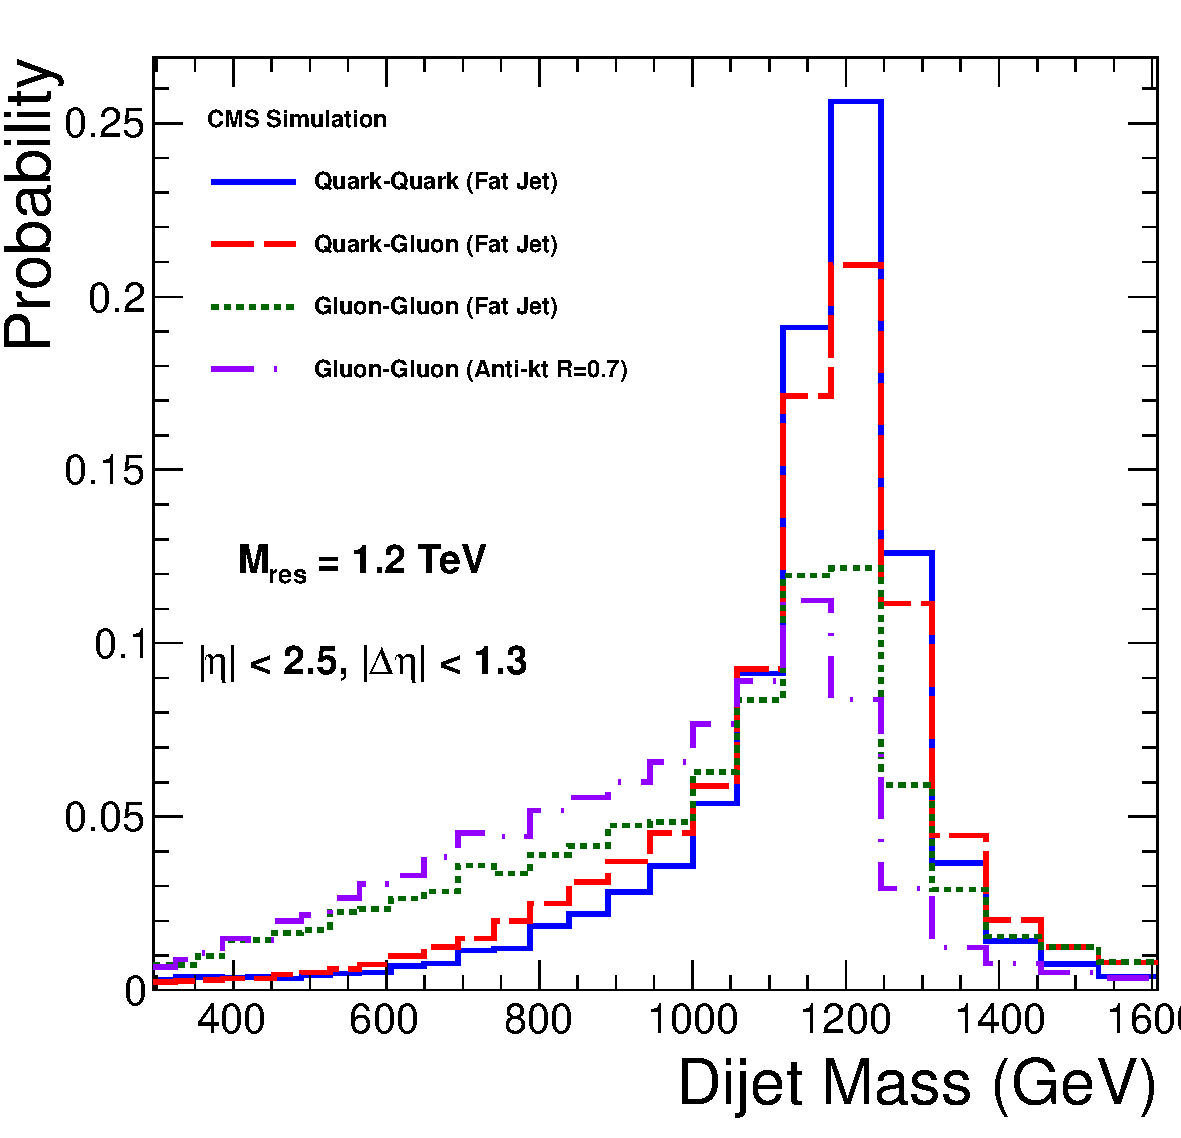
\includegraphics[width=0.45\textwidth]{Figures/shape_1200GeV.pdf}
       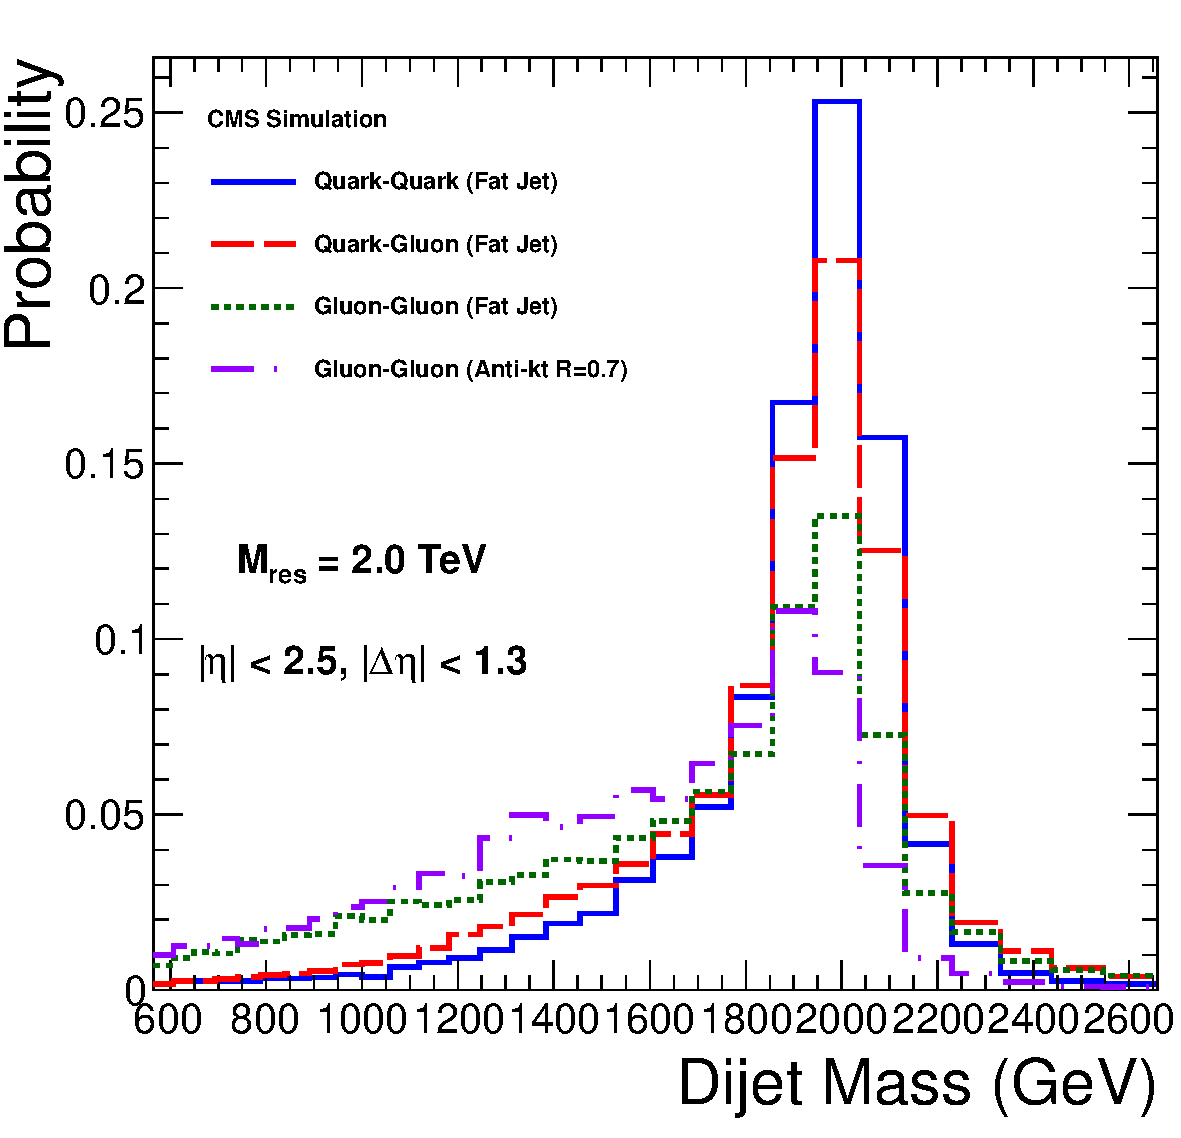
\includegraphics[width=0.45\textwidth]{Figures/shape_2000GeV.pdf}
        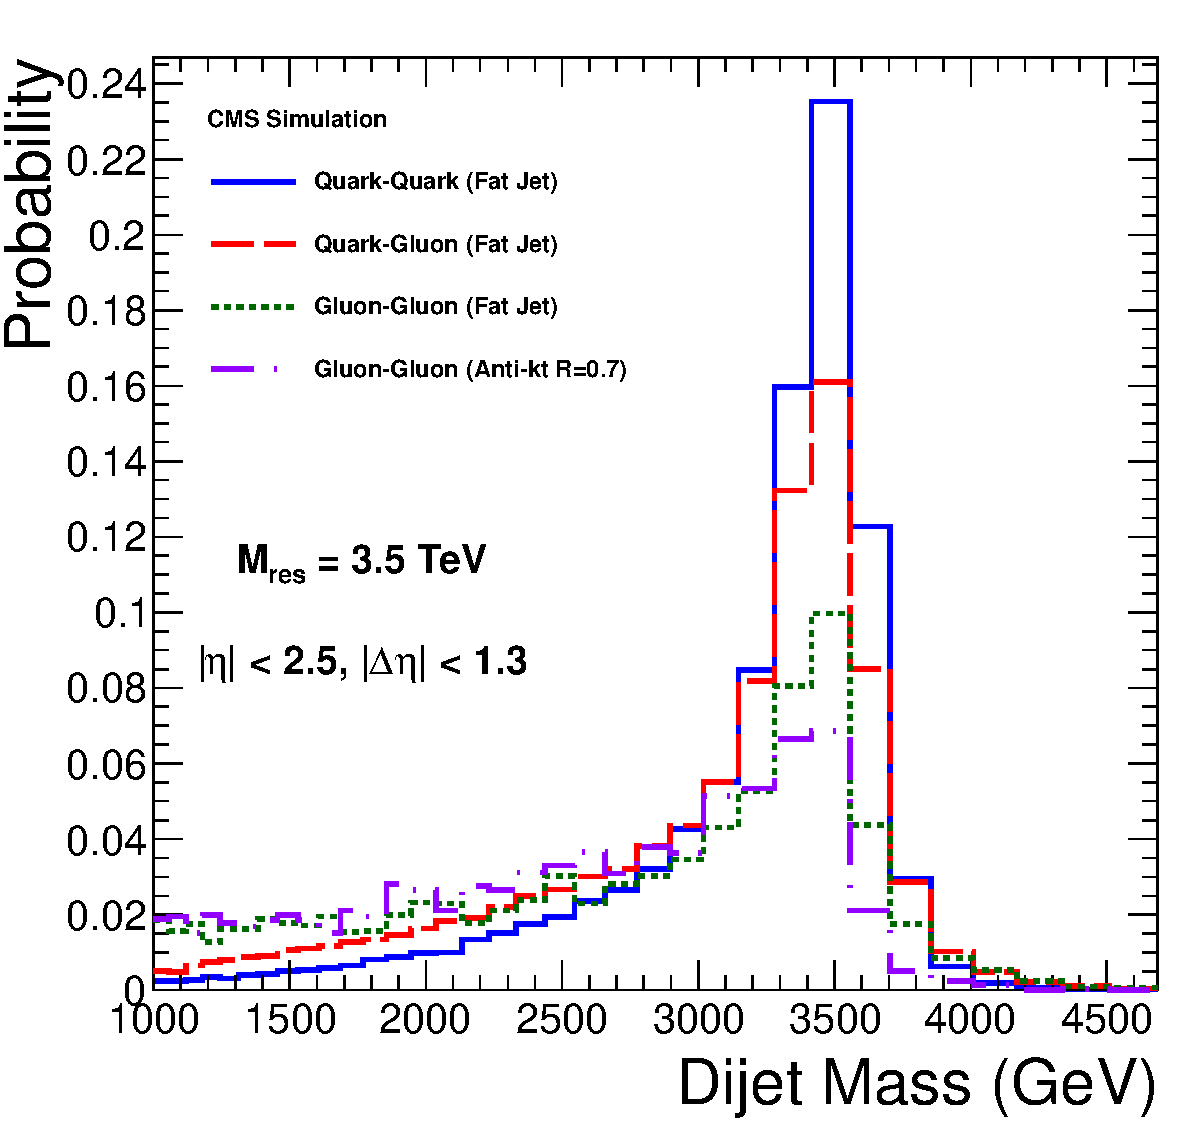
\includegraphics[width=0.45\textwidth]{Figures/shape_3500GeV.pdf}
    \caption{Dijet mass distribution for $q\bar{q}$ $(qq)$, $qg$ and $gg$ resonances at 
    $0.5$, $0.7$, $1.2$, $2$ and $3.5$ TeV resonance mass.}
    \label{resonance_shape}
  \end{center}
\end{figure}



We search for narrow dijet resonances in general, rather 
than a specific model of dijet resonance production.


We require only a model of the resonance line shape. We will only 
consider narrow resonances in this analysis, for which the
natural resonance width is negligible compared to the CMS dijet mass 
resolution, so that the natural width does not affect the resonance shape.
The type of parton pairs in the resonance decay ($qq$, $qg$, or $gg$)
does affect the resonance shape.  To obtain generic shapes for these three
types of parton pairings, the process of $qg\rightarrow q*\rightarrow qg$, 
$q\bar{q} \rightarrow G\rightarrow q\bar{q}$ and 
$gg \rightarrow G\rightarrow gg$ were produced using 
PYTHIA+CMS Spring10 simulation at five different masses of $0.5$, $0.7$, 
$1.2$, $2$ and $3.5$ $TeV$. In Fig.~\ref{resonance_shape} we present four of
these five resonance shapes.



  The source of the shape differences among $qq$, $qg$ and $gg$ resonances 
has been studied previously~\cite{CMS_AN_2009-145}.
The width of dijet resonances increases with the number of gluons in the 
final state, primarily
because gluons emit more radiation than quarks.  The peak value of dijet mass of
the resonance decreases with the number of final state gluons, primarily due 
to smaller response of the CMS detector to gluon jets than to quark jets. 
The low mass tail of the resonance shape comes primarily from final state 
radiation. A small high mass tail comes from initial state radiation. 
These resonance shapes are approximately valid for any model of resonance 
involving these pairs of partons, assuming the models natural half-width 
($\Gamma / 2$) is small compared to the dijet mass resolution.  In 
Fig~\ref{resolution} we present an estimate of the resolution of the Gaussian 
core of the dijet mass response distribution from fits to the peak in an 
interval between $-0.5\sigma$ and $1.5\sigma$.  


\begin{figure}[hbt]
  \begin{center}
     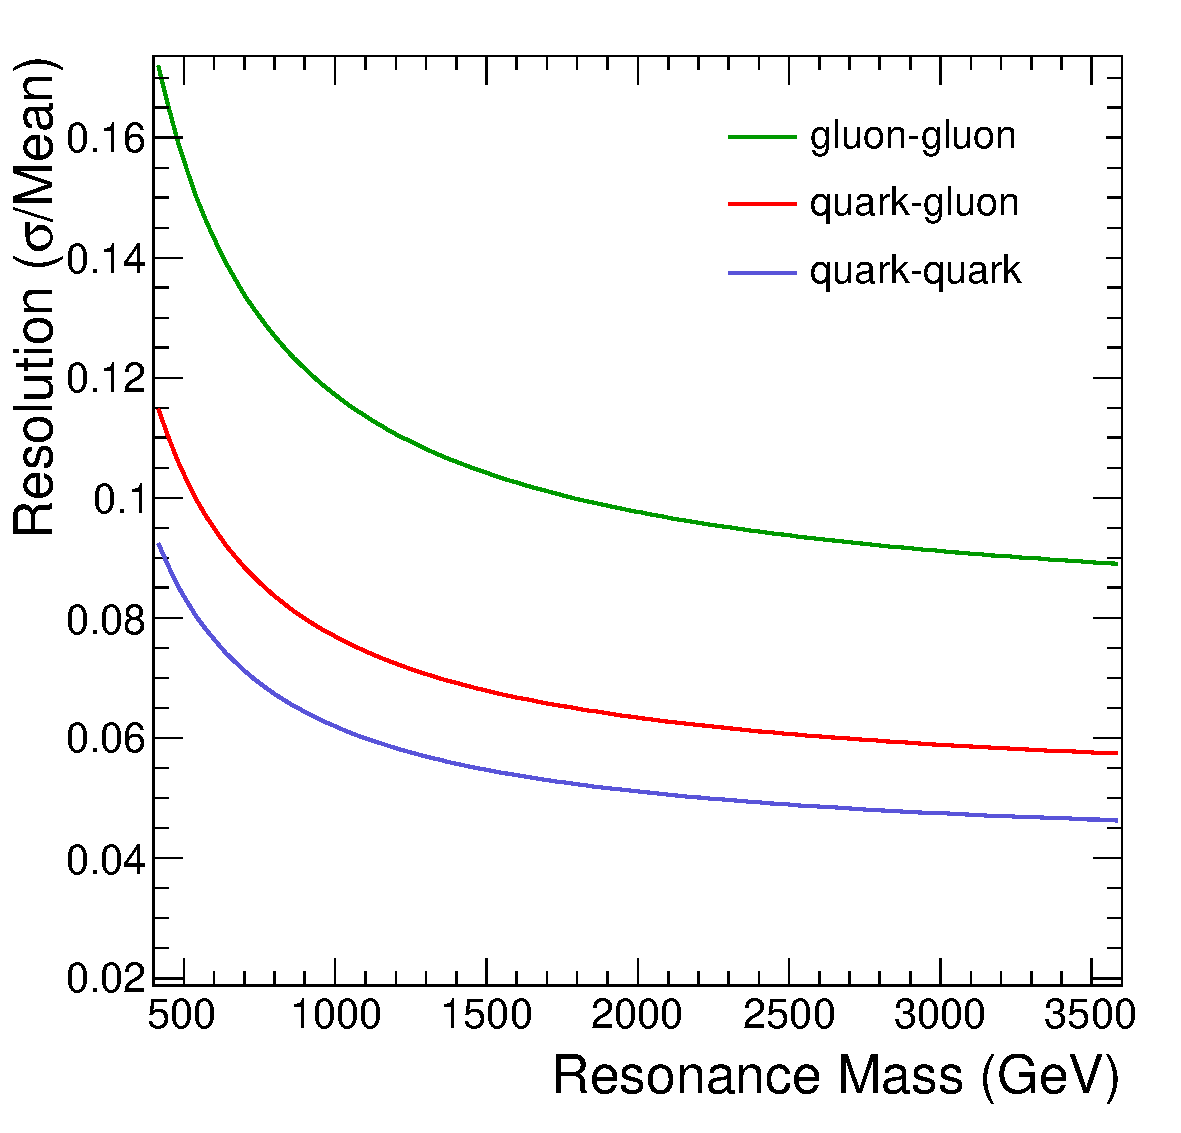
\includegraphics[width=\textwidth]{Figures/Comp_resolution_Color.pdf}
     \caption{The fractional width of the Gaussian core of the response distribution 
     as a function of resonance mass from CMS detector simulations of 
      $qq$, $qg$ and $gg$ dijet resonances.  }
    \label{resolution}
  \end{center}
\end{figure}

Fig.~\ref{shape} shows the simulated signal of excited quark.
The resonance shape at resonance masses of $M=0.5$,$0.7$, $1.2$, $2.0$ and $3.5$
TeV were obtained from simulation.
We obtain the resonance shapes at intermediate masses via an 
interpolation technique~\cite{CMS_AN_2009-070}. For example the $1.5$ TeV
shape shown in Fig.~\ref{shape} comes from interpolation. The interpolation 
technique
has been checked by doing a wider interpolating between $M=0.7$ and $2.0$ TeV to get the $1.2$ TeV resonance
and comparing that with the actual simulation, and the shapes were the same. 
We use the resonance shapes from our interpolation technique to calculate the cross 
section upper limit at any resonance mass.

\begin{figure}[hbt]
  \begin{center}
     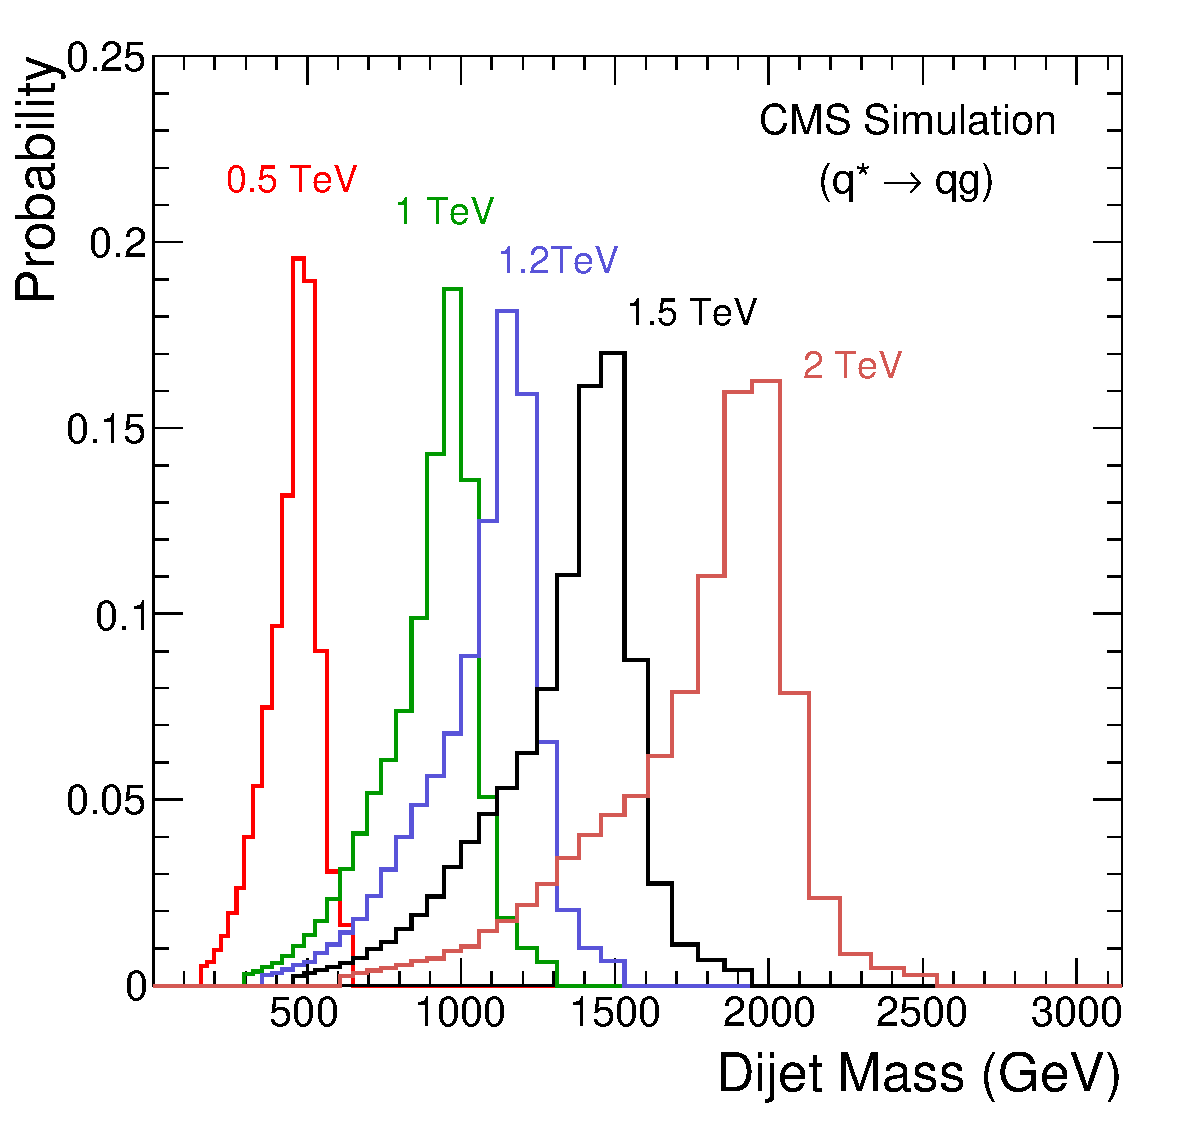
\includegraphics[width=\textwidth]{Figures/Shapes_qg.pdf}
     \caption{$qg$ resonance shapes at various resonance masses coming
     from excited quark simulation at resonance masses in TeV of 
     $0.5$ (red), $0.7$ (green), $1.2$ (blue), $2.0$ (red) and $3.5$ (not shown) and interpolation
     at the example mass of $1.5$ TeV (black).}
    \label{shape}
  \end{center}
\end{figure}

Fig.~\ref{signal} shows the differential 
cross section of excited quark signals as a function of dijet mass 
superimposed on the plot of the dijet mass data with background fit. 
Fig.~\ref{signal} also shows the 
differential cross section of string resonance signals. We model the
string resonance line shape using the excited quark shape since 
string resonances decay predominantly to a
quark and a gluon (see appendix~\ref{appString}) like the excited 
quark. Fig.~\ref{signal} demonstrates that the expected string 
resonance cross section is large, much greater than our measured data.
%The fractional difference between the data and the smooth
%background fit is compared to 
%simulated excited quark resonance signals in Fig.~\ref{fract_signal}, and
%to string resonance signals in Fig.~\ref{fract_signal_string}.  Note 
%the vertical scales are different in Fig.~\ref{fract_signal} and 
%Fig.~\ref{fract_signal_string}.  
In Fig.~\ref{DataOverFit} we show the ratio
between the data and the fit compared to simulated signals for both excited
quarks and string resonances.

\begin{figure}[hbt]
  \begin{center}
     \includegraphics[width=\textwidth]{Figures/DijetMass_withSignal_string.pdf}
     \caption{The dijet mass distribution (points) compared to a smooth
     background fit (blue solid curve) and to a simulation of
     excited quarks (red dot-dashed curves) and string resonances (green dashed
     curves) in the CMS 
     detector.}
    \label{signal}
  \end{center}
\end{figure}

%\begin{figure}[hbt]
%  \begin{center}
%     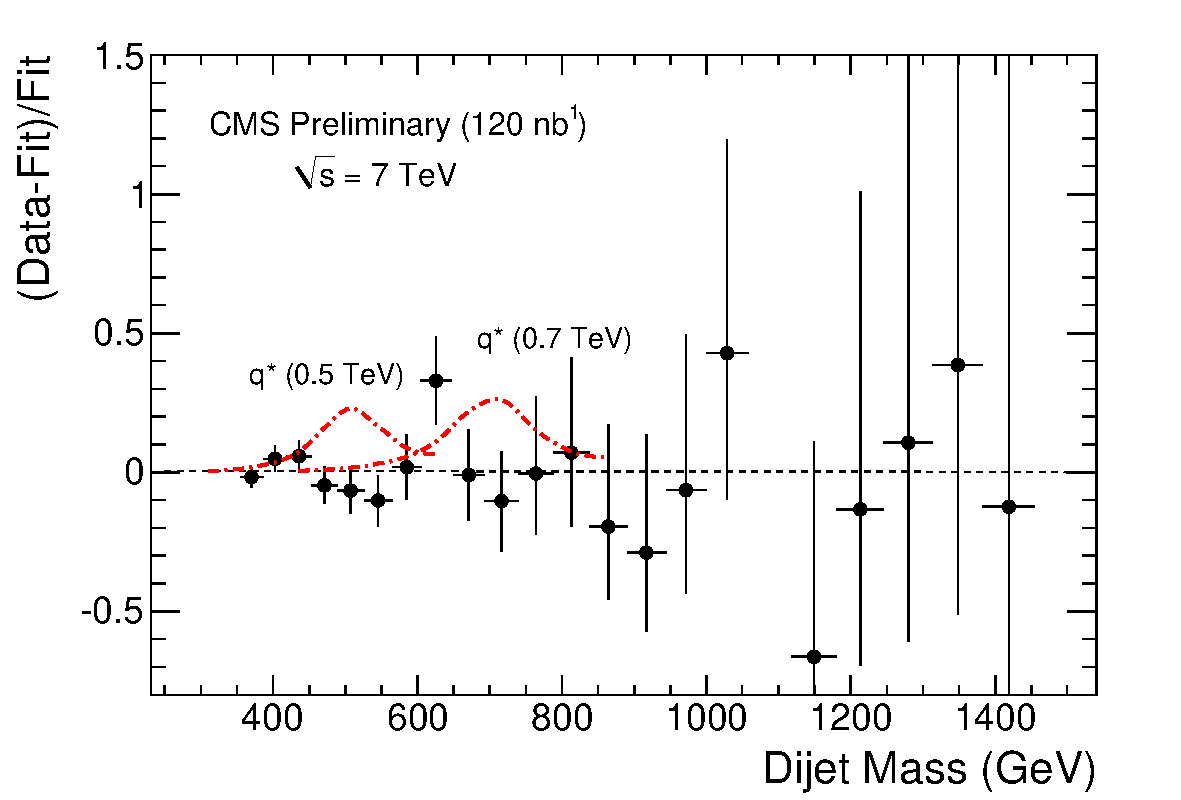
\includegraphics[width=\textwidth]{Figures/Fract_change_withsignal.pdf}
%     \caption{ The fractional difference between the dijet mass distribution (points) and a smooth
%background fit (dashed line) is compared to simulations of excited quark signals in the CMS
%detector (dot-dashed red curves).}
%    \label{fract_signal}
%  \end{center}
%\end{figure}

%\begin{figure}[hbt]
%  \begin{center}
%     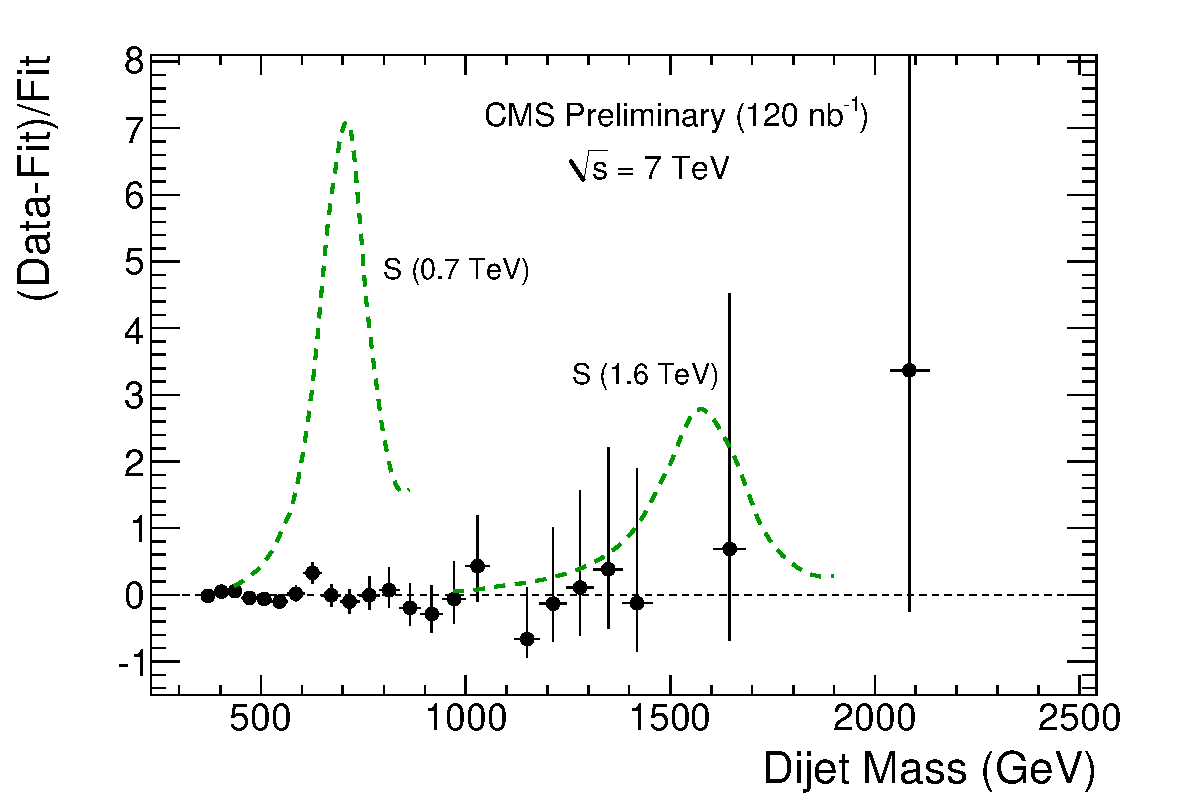
\includegraphics[width=\textwidth]{Figures/Fract_change_withsignal_string.pdf}
%     \caption{ The fractional difference between the dijet mass distribution (points) and a smooth
%background fit (dashed line) is compared to a simulation of a string resonance signal in the CMS
%detector (dashed green curve).}
%    \label{fract_signal_string}
%  \end{center}
%\end{figure}


\begin{figure}[hbt]
  \begin{center}
     \includegraphics[width=\textwidth]{Figures/Fractional_Diff_AllSignal.pdf}
     \caption{ The ratio between the dijet mass distribution (points) and a smooth
background fit (dashed line) is compared to a CMS detector simulation of an excited quark signal (dashed red curve) and
a string resonance signal (dashed green curve).}
    \label{DataOverFit}
  \end{center}
\end{figure}


\clearpage

\subsection {Largest Fluctuation and Significance}
\label{significance}
The search range of Dijet mass is not well defined since there is no prediction for the Dijet 
Resonance mass(es).  Therefore the probability to find upward fluctuation is increased by searching for 
resonance(s) anywhere and we need to take the ``Look Elsewhere Effect'' into account.  
A MC simulation is used to estimate the significance of a resonance possibly to be observed in data.
The biggest  fluctuation in the current dataset (2875.0 nb$^{-1}$) (Search window: between 500 and 2000 GeV) 
is used to illustrate the method.


Two fits to the data are defined as: the null-hypothesis fit is a fit to the data using background 
model only and the signal-hypothesis fit is a fit to the data using background model and a signal 
model together. The likelihood ($\chi^2$) returned from the null- or signal-hypothesis fit  is denoted 
as $L_0$ ($\chi^2_0$) or $L_S$ ($\chi^2_S$).  The $\sqrt{-2\Delta ln}=\sqrt{-2ln(L_0/L_S)}$ or 
$\sqrt{-\Delta \chi^2}=\sqrt{\chi^2_0-\chi^2_S}$ value is called the local significance and 
will be used to determine the significance including the ``Look Elsewhere Effect''.
Fig.~\ref{nullfit} and ~\ref{signalfit} show the null- and signal-hypothesis fit, 
with the lowest $\chi^2$ at $q^*$ mass of 900 $GeV/c^2$ in the search range of 500 to  
2000 $GeV/c^2$, to the current dataset  (2875.0 $\mathrm{nb}^{-1}$) with a local 
significance of 1.7 obtained by $\sqrt{\Delta \chi^2}=\sqrt{5.29}$ assuming
one degree of freedom.  
And Fig.~\ref{signalshape} shows the fractional 
background subtracted Dijet mass from the signal-hypothesis fit with a $q^*$ fluctuation shape.



To estimate the probability that background fluctuations alone would give rise to signals (fluctuations) 
as significant as that seen in the data, we simulate Dijet mass spectra based on the background 
distribution alone, and search for the most significant fluctuation in each spectrum in the mass range 
of 500 to 2000 $GeV/c^2$, with the $q^*$ mass shape at various resonance masses. In this case, a total 
number of  414131 events (match to the total number of events in the data) is generated for each trial.
From these simulated spectra we obtain the distribution for the quantity��${-\Delta \chi^2}$ 
in pure background samples, and compare this with the signal (fluctuation in this dataset) in the data. 
We performed a total of 100 and found 40 trials with a ${-\Delta \chi^2}$ value greater than 
or equal to the value obtained in the data as shown in Fig.~\ref{toy2dln}. The p-value obtained from 
MC simulation is 40\%, corresponding to a significance of 0.2$\sigma$. Thus, the significance is decreased from 
1.7$\sigma$ to 0.2$\sigma$ by taking the ``Look Elsewhere Effect'' into account.



\begin{figure}[hbt]
  \begin{center}
     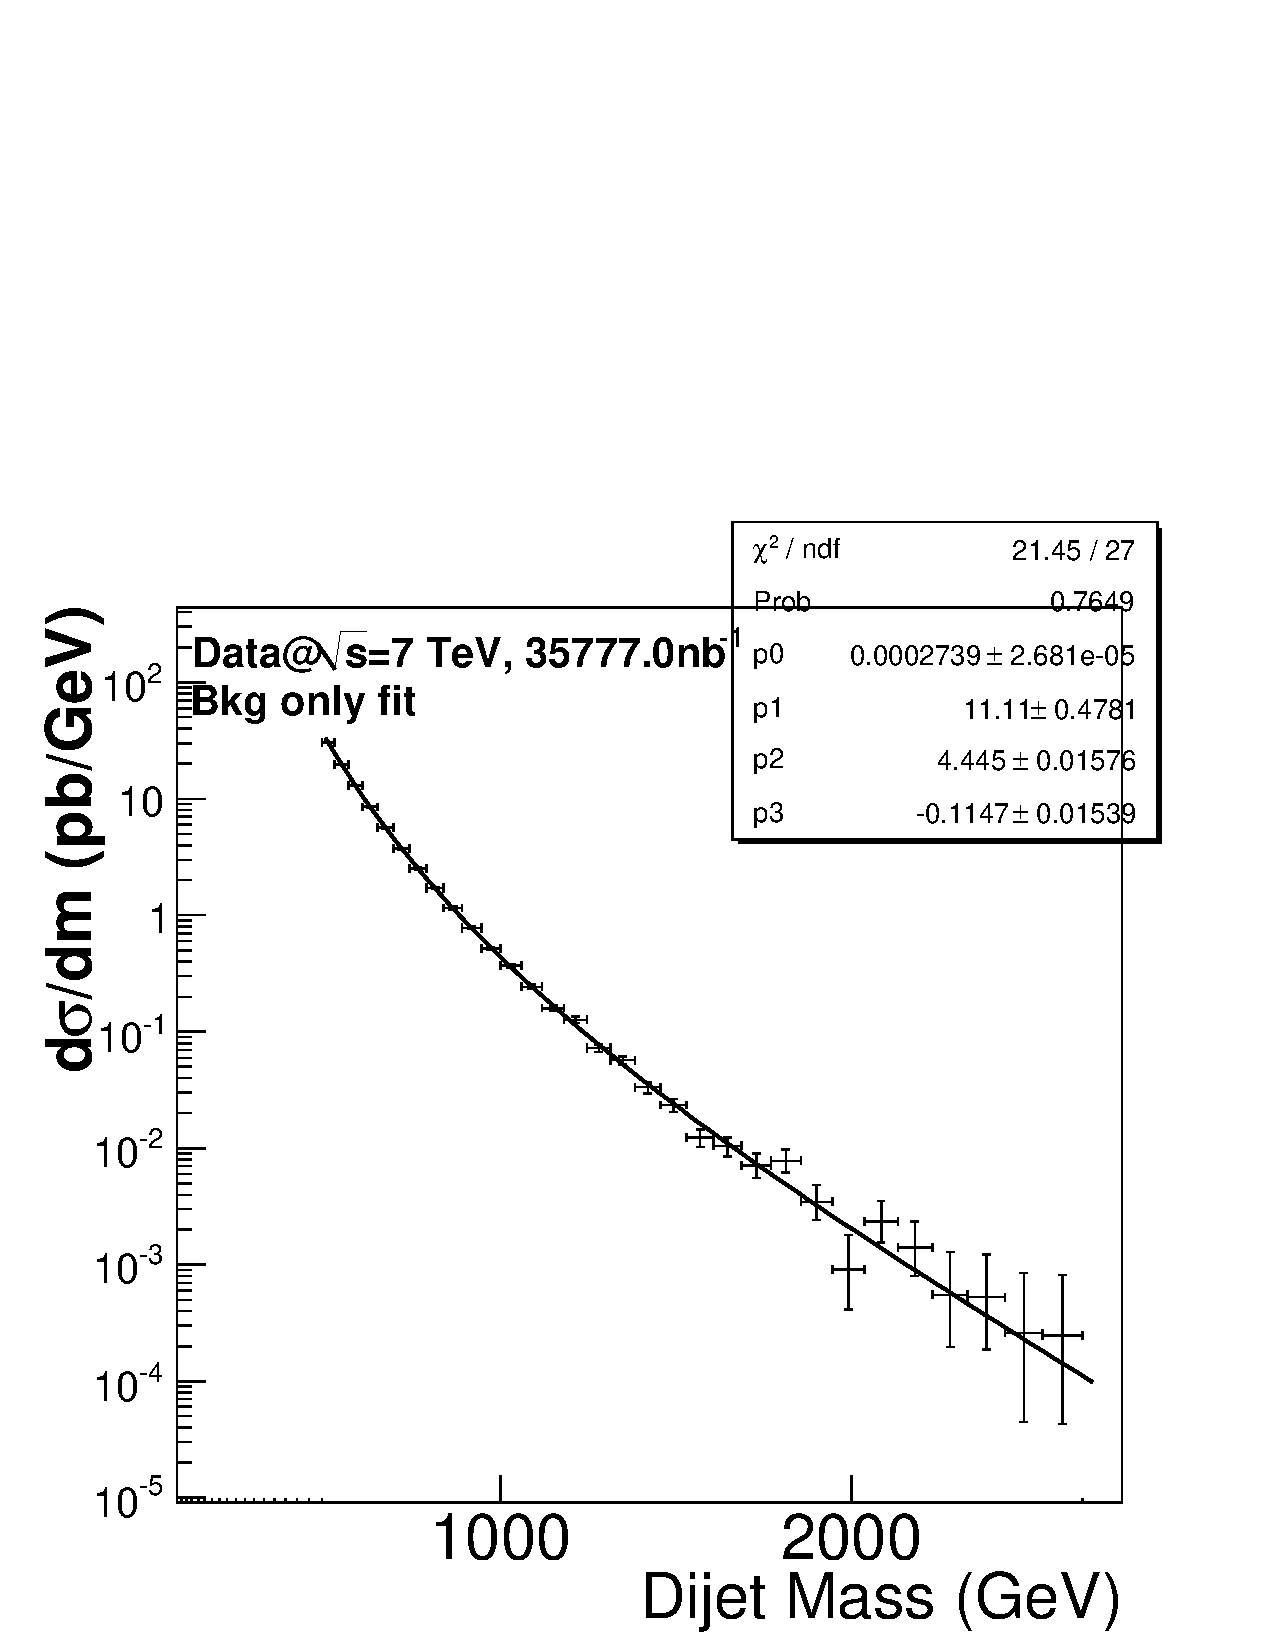
\includegraphics[width=\textwidth]{Figures/nullhypothesisfit.pdf}
     \caption{The null-hypothesis fit to the Dijet mass in the current dataset using 
equation~\ref{eqParam}.
}
    \label{nullfit}
  \end{center}
\end{figure}

\begin{figure}[hbt]
  \begin{center}
     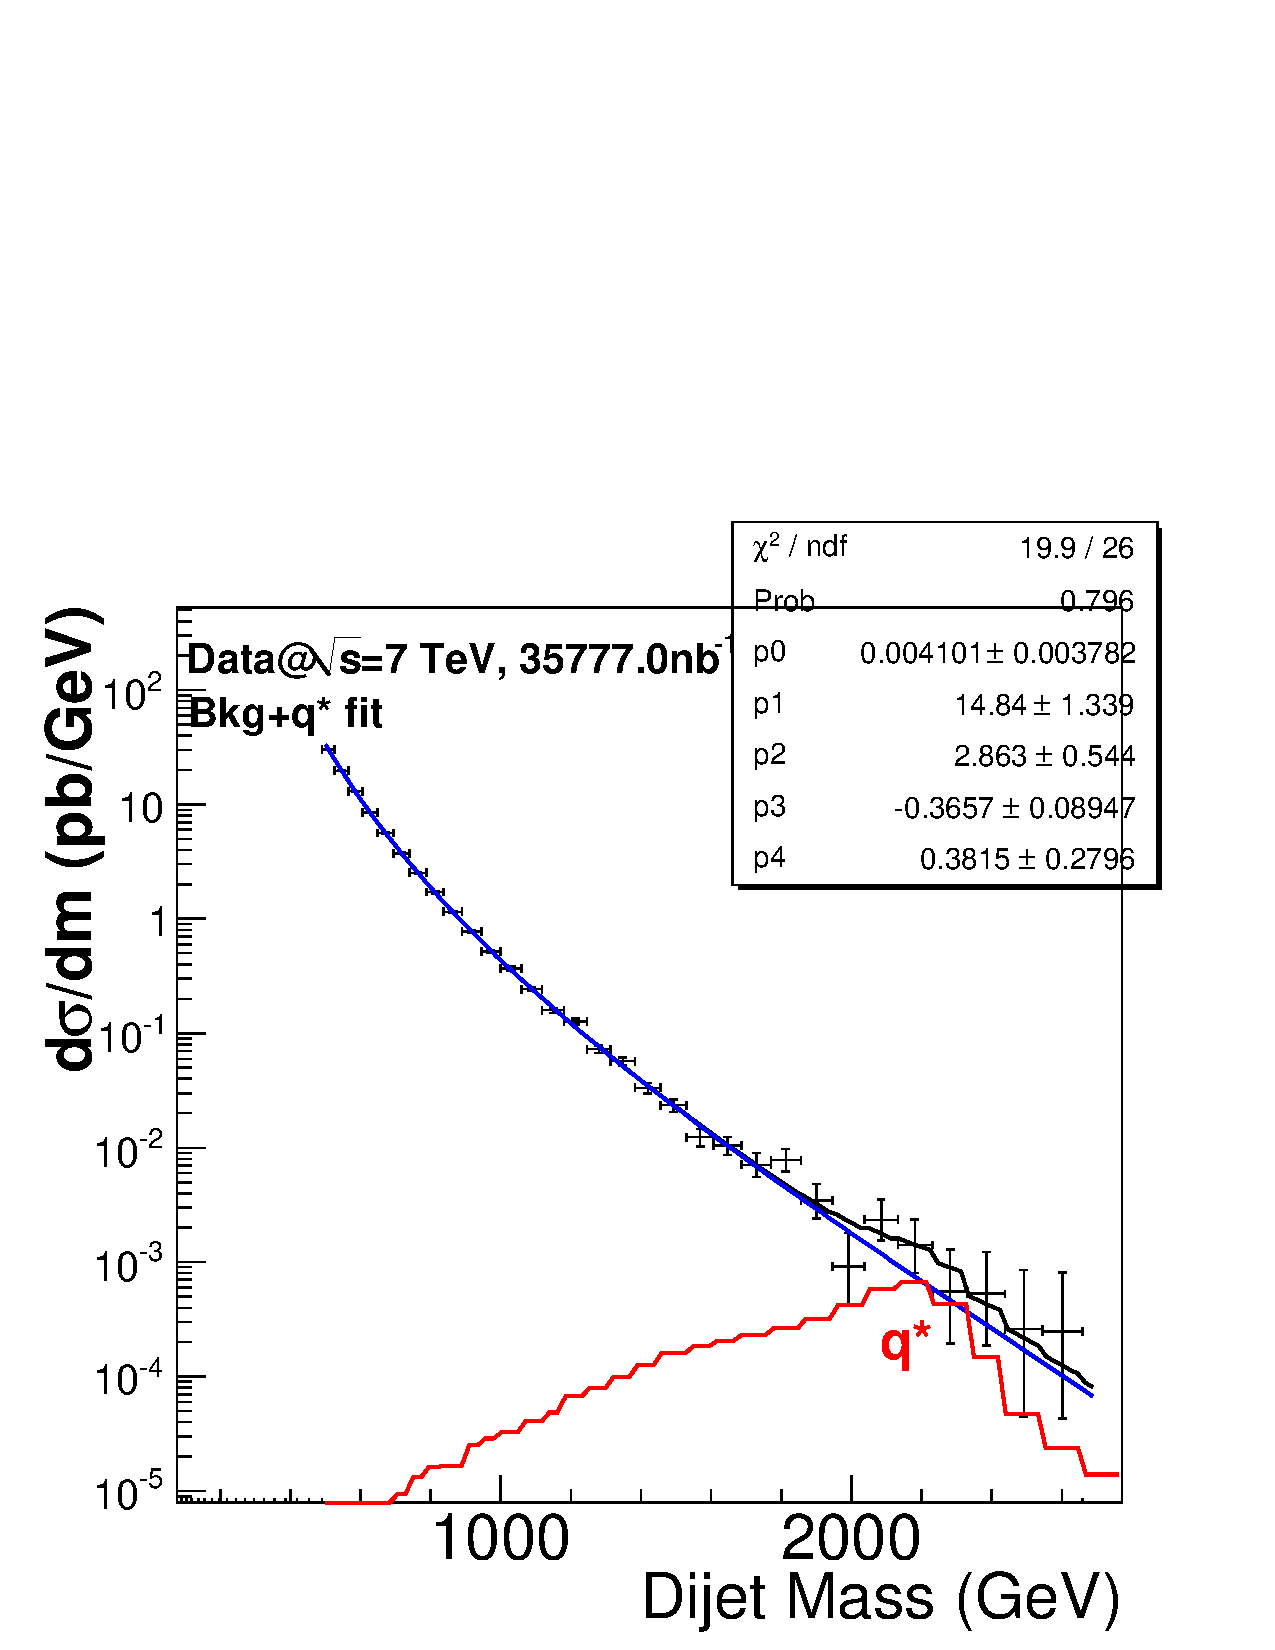
\includegraphics[width=\textwidth]{Figures/signalhypothesis.pdf}
     \caption{The signal-hypothesis fit to the Dijet mass in the current dataset using 
equation~\ref{eqParam} and $q^*$ resonance shape.
}
    \label{signalfit}
  \end{center}
\end{figure}


\begin{figure}[hbt]
  \begin{center}
     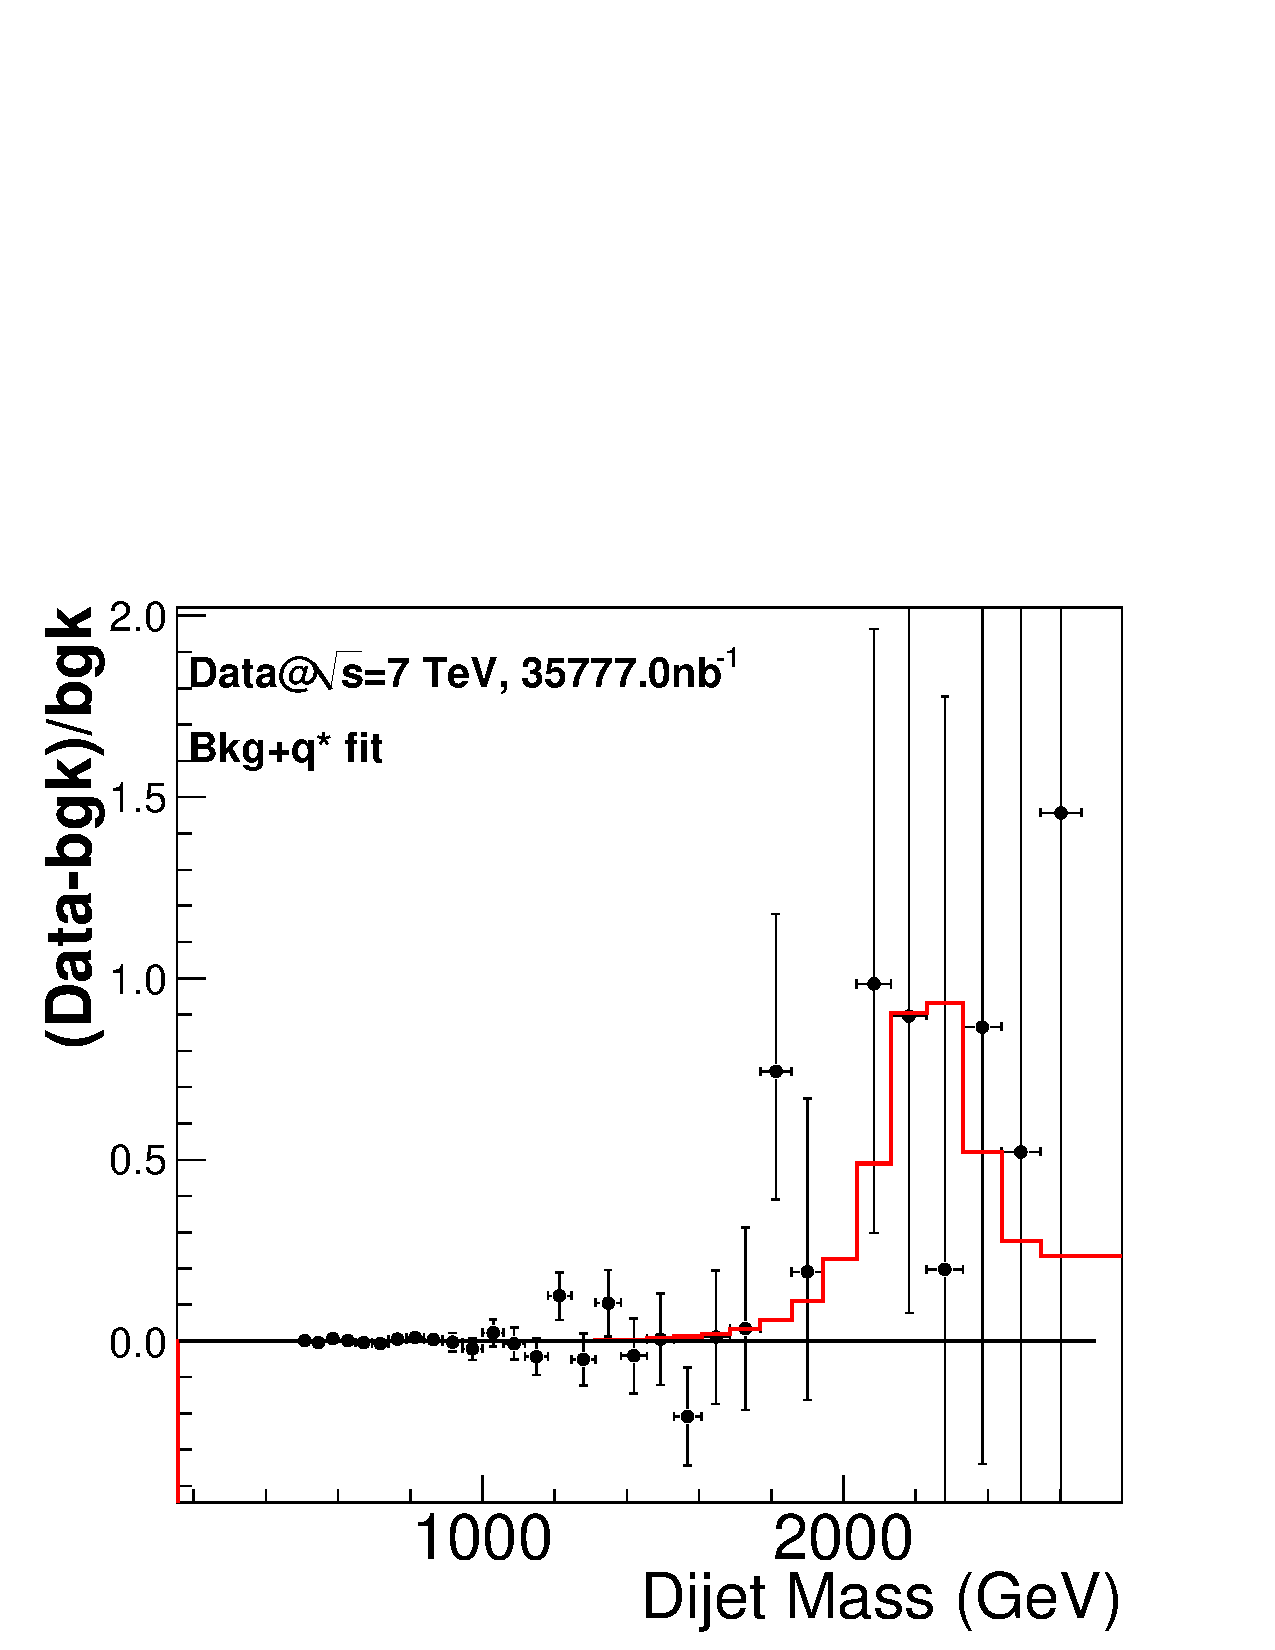
\includegraphics[width=\textwidth]{Figures/signalhypothesisQstarresidual.pdf}
     \caption{The fractional background subtracted Dijet mass from the signal-hypothesis fit.
}
    \label{signalshape}
  \end{center}
\end{figure}

\begin{figure}[hbt]
  \begin{center}
     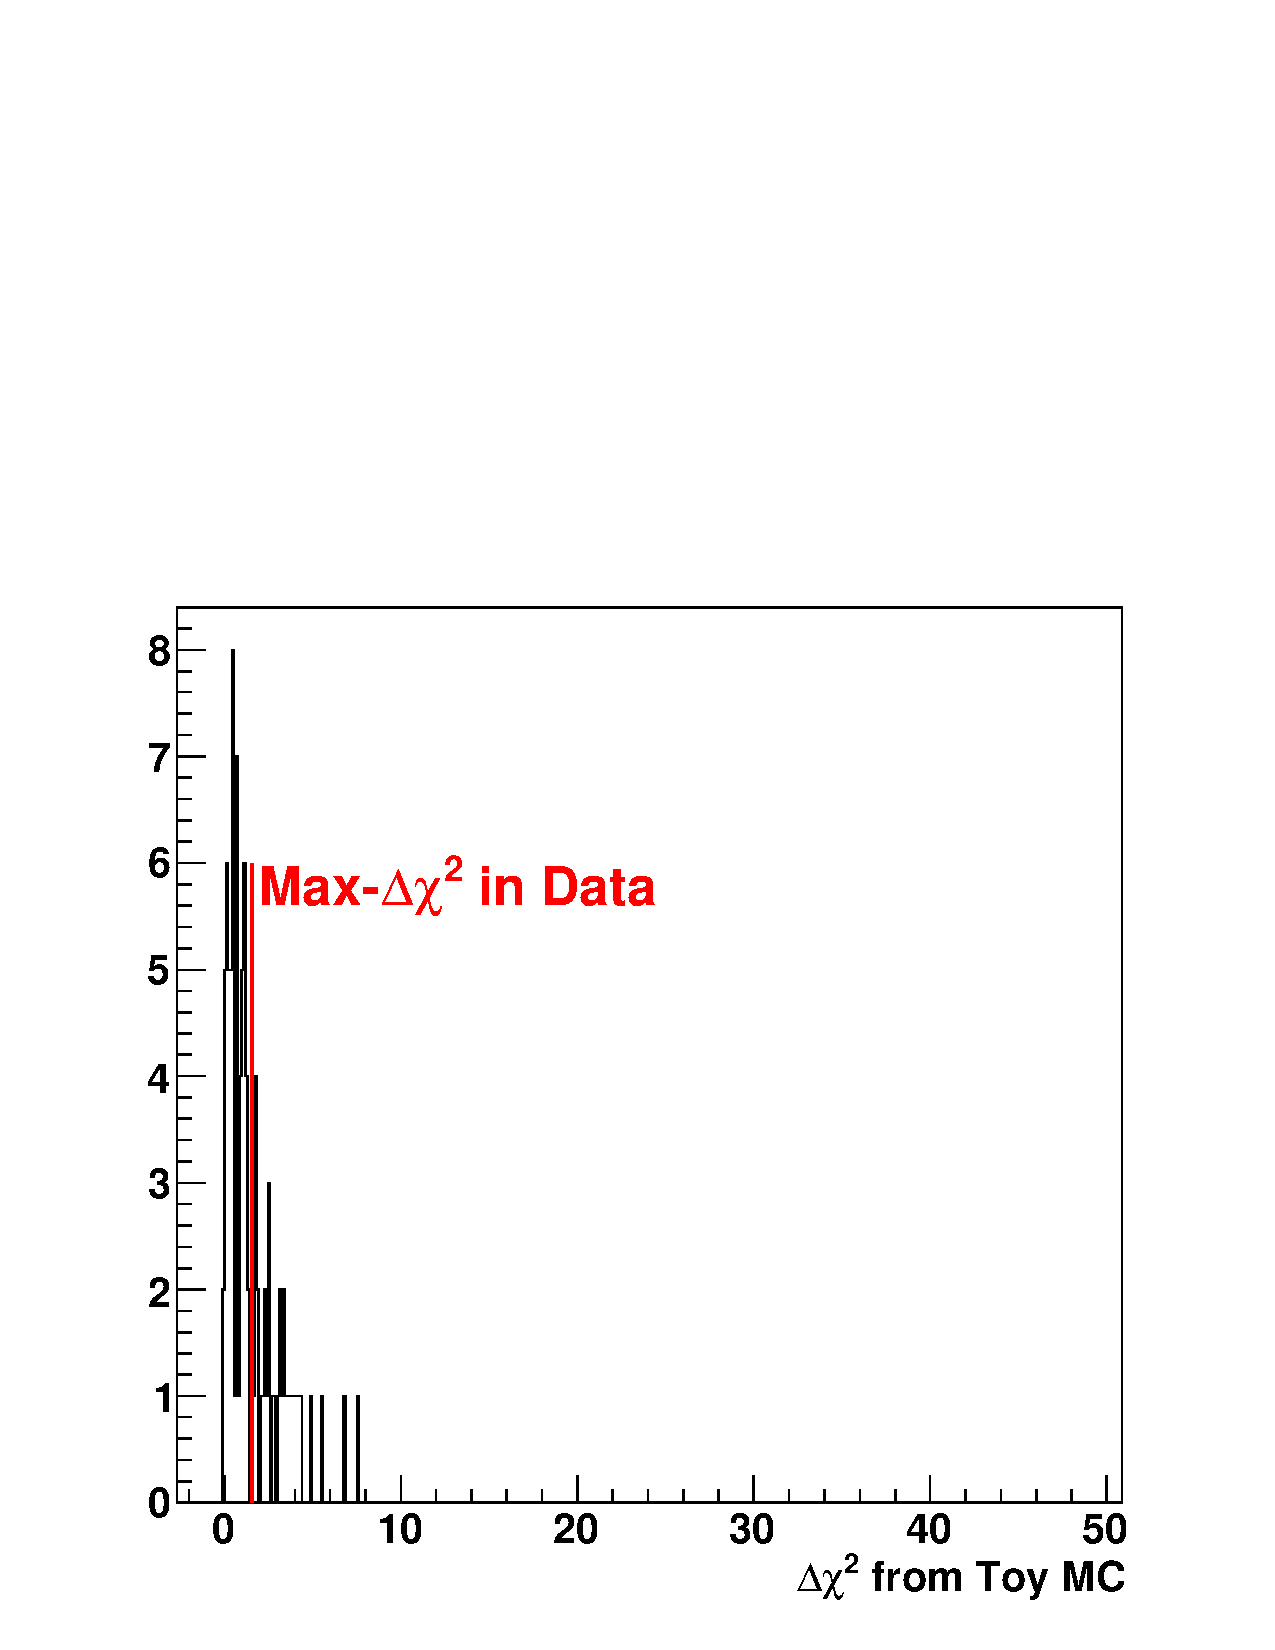
\includegraphics[width=\textwidth]{Figures/toychisq.pdf}
     \caption{The $-\Delta \chi^2$ distribution obtained from MC simulation.
} 
   \label{toy2dln}
  \end{center}
\end{figure}



\clearpage

%\subsection {Angular distributions of Largest Fluctuation}

%Bumps observed in the data that arise from resonance production 
%should also produce deviations in the dijet angular distributions.
%The companion dijet centrality ratio analysis gives us a single 
%measure of the dijet angular distribution for such a resonance~\cite{CMS_AN_2010-126}.
%For the 3 events around 1.3 TeV shown and tabulated in Appendix~\ref{appEvents},
%there is one "inner" dijet inside with both jets satisfying $|\eta|<0.7$,
%and one "outer" dijet with both jets satisifying $0.7<|\eta|<1.3$, for
%a dijet ratio of 1 with an upper statistical error of 10 and a lower statistical
%error of $0.9$ (Clopper Pearson errors).
%For QCD we would expect about $0.5$ and for a resonance we would expect 
%between 2.5 and 4 depending on resonance type.  With this low
%statistics the dijet ratio fro the dtata is compatible with both QCD and a resonance,
%and does not tell us much.
%

%In addition to the dijet ratio, we can look in detail at the $\eta$ and $\cos\theta^*$
%distributions shown in Fig.~\ref{anglesForBump}.  Here we have plotted for the 3 events
%around a dijet mass of $1.3$ TeV the $\eta$ of 
%each of the two leading jets and compared it with the predictions of both QCD and
%a nearby resonance simulation at 1.2 TeV.  The data is compatible with either for these
%low statistics, but looks a little more like QCD, particularly for the $\cos\theta^*$
%distribution.  The angular distributions do not support a resonance
%hypothesis for the 3 events near 1.3 TeV.


%\begin{figure}[hbt]
%  \begin{center}
%     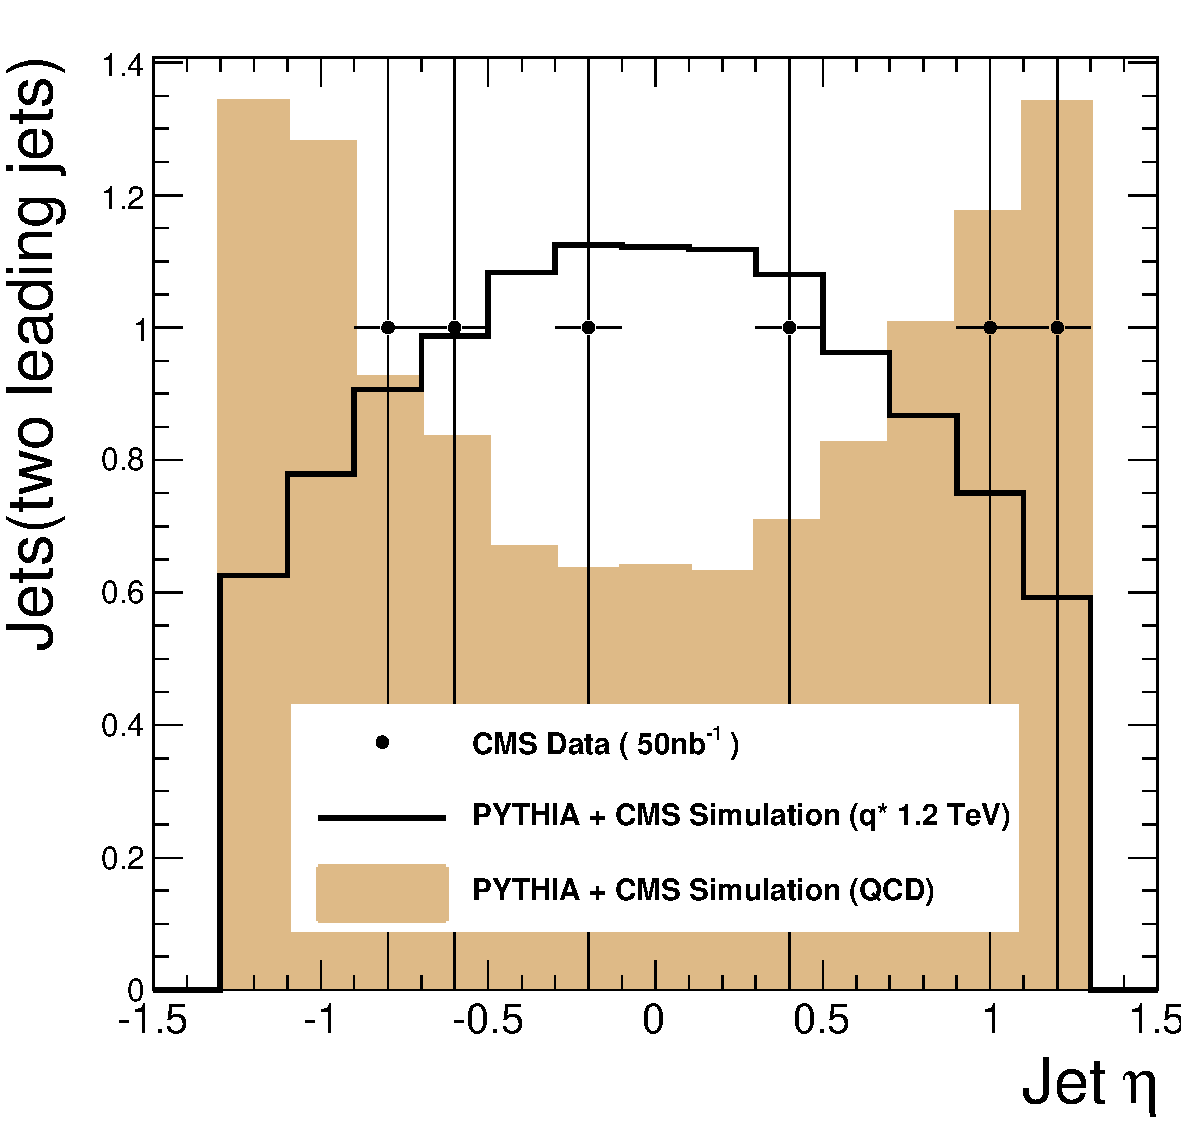
\includegraphics[width=0.48\textwidth]{Figures/c_EtaWithResonance.pdf}
%     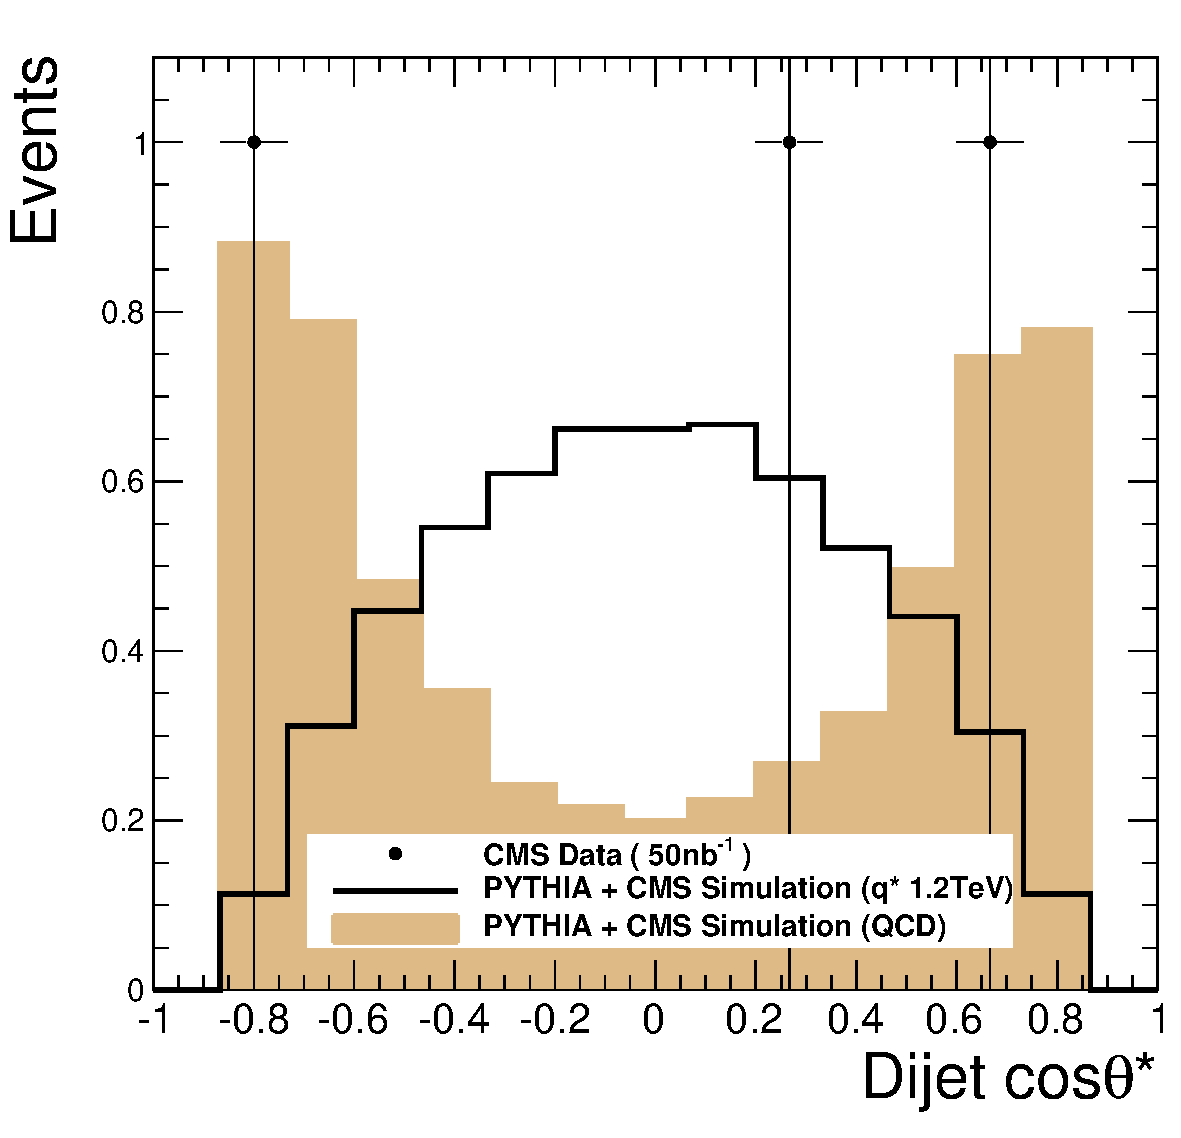
\includegraphics[width=0.48\textwidth]{Figures/c_CosThetaStar.pdf}
%     \caption{The jet $\eta$ (left) and the dijet $\cos\theta^*$ (right) for the three events
%     in the data near 1.3 TeV (points) is compared to the QCD prediction for dijet mass in 
%     the range 1.2-1.5 TeV (filled histogram) and an excited quark resonance simulation
%     (black histogram).} 
%   \label{anglesForBump}
%  \end{center}
%\end{figure}


%\clearpage

\subsection{Angular Ratio vs. Dijet Mass}
\label{sectionAngle}
In Fig.~\ref{jet_kinematics} we showed the dijet $\Delta\eta$ 
distribution for $m<220$ GeV.  This is a measure of the center of 
momentum frame dijet angular distribution. It peaks at high 
$\Delta\eta$ for QCD, and at low $\Delta\eta$ for new physics.
We construct the following ratio
\begin{equation}
\frac{N(|\Delta\eta|<0.7)}{N(0.7<|\Delta\eta|<1.3)}
\end{equation}
as a  simple measure of the dijet angular distribution within each
of our dijet mass bins, and plot as a function  of mass in 
Fig.~\ref{figAngularRatio}. The data compares well with a QCD prediction
from PYTHIA and the CMS simulation scaled by an overall factor to match the 
data on average. This indicates there is no evidence of new physics
in the angular distribution, and the angular distribution is roughly what
we expect from QCD. The high fluctuation studied in the last section does
not show an angular ratio greater than expected in this distribution.
\begin{figure}[!ht]
  \begin{center}
        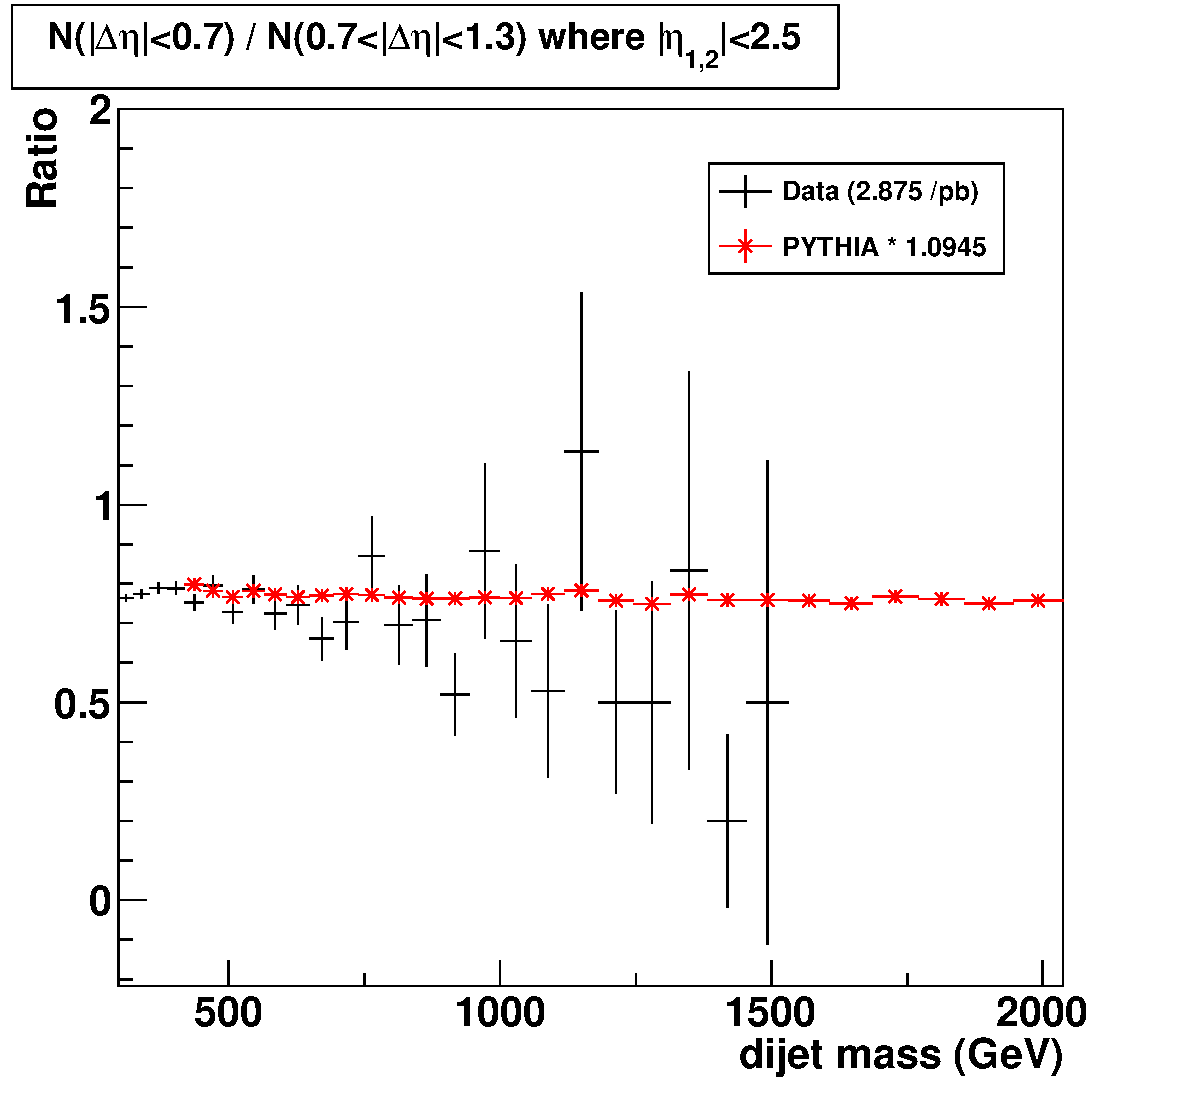
\includegraphics[width=0.8\textwidth]{Figures/DijetRatio}
    \caption{ Angular distribution ratio as a function of dijet mass from data
    and (black points) and a QCD simulation normalized to the data (red points
    and curve)}
    \label{figAngularRatio}
  \end{center}
\end{figure}
\clearpage

\subsection {Setting Cross Section Upper Limits}

For setting upper limits, before accounting for systematic uncertainties,
we begin with a Bayesian formalism with uniform prior for the cross section.
The binned likelihood, L, as a function of a constant $\alpha$ can be written as:
\\
\begin{equation}
L = \prod_{i} \frac{\mu_{i}^{n_{i}}e^{-\mu_{i}}}{n_{i}!}
\end{equation}
\\
where
\\
\begin{equation}
\mu_{i} = \alpha N_{i}(S) + N_{i}(B).
\end{equation}
\\
$n_{i}$ is measured number of events in the $i-th$ dijet mass bin, $N_{i}(S)$ is number of events from signal in the $i-th$ dijet mass bin,
$\alpha$ is a constant to multiply the signal and $N_{i}(B)$ is number of expected events from background in the $i-th$ dijet mass bin.
We consider that QCD background is fixed to the best $Signal+QCD$ fit to data point and it gives the expected number of background event in the $i-th$
dijet mass bin,$N_{i}(B)$. The number of signal in the $i-th$ dijet mass bin,$N_{i}(S)$,comes from developed interpolation technique.
The signal range is chosen from $0.3\cdot M_{Res}$ to $1.3\cdot M_{Res}$ an interval which contains nearly all the resonance
line shape.
We assume a flat prior in $\alpha$, which is the same as a flat prior in the resonance cross section.  With this assumption
the likelihood normalized to unity is equivalent to a posterior probability density, and can be used to set limits.  
We calculate the posterior probability density as a function of signal cross section for resonances with 
mass from $0.5$ TeV to $2.6$ TeV in $0.1$ TeV steps.  We show them in  Appendix~\ref{appLike} for qg resonances.
The 95\% confidence level upper limit is calculated from the posterior probability density as follows;

\begin{equation}
\frac{\int_{0}^{\sigma_{95}} P_{POST}(\sigma)d\sigma}{\int_{0}^{\infty} P_{POST}(\sigma)d\sigma} = 0.95
\end{equation}

%In Fig.~\ref{Likelihood}, Likelihood distribution at $0.7$ GeV resonance masses for $qg$ resonances are illustrated. The likelihood distributions 
%for resonance mass from $0.5$ TeV to $1.5$ TeV in $0.1$ TeV step can be seen in Appendix X.
%
%\begin{figure}[!ht]
%  \begin{center}
%    \includegraphics[width=0.55\textwidth]{Figures/Likelihood_700GeV.pdf}
%    \caption{Likelihood Distribution with statistical error only.}
%    \label{Likelihood}
%  \end{center}
%\end{figure}


We present 95\% CL upper limit on dijet resonance cross section in 
Fig.~\ref{Limit_statonly} including only statistical uncertainties. 
Quark-quark, quark-gluon and gluon-gluon 
resonances are shown separately. The limits have small wiggles 
corresponding to structures in the data, and the width of the
resonance line shape.  
The limits are also tabulated in table~\ref{tabStatLimit}. 
At the highest resonance mass shown,
2.6 TeV, the limits have a value of between 4 and 6 events corresponding to 
the few events observed on the tail of the dijet mass distribution that are 
still within the resonance line shape.  
In prior analysis versions, where there were no events 
at high dijet mass, we have shown explicitly that the limit plateaus at exactly 3 
events corresponding to 0 events observed.  

\begin{figure}[!ht]
  \begin{center}
    \includegraphics[width=\textwidth]{Figures/Limit_Comp_statonly.pdf}
    \caption{Dijet resonance sensitivity with statistical errors only. 95\% C.L. upper limit on cross section 
    is compared to the cross section for various resonance models.
This sensitivity does not contain estimates of the systematic uncertainties.}
    \label{Limit_statonly}
  \end{center}
\end{figure}


The procedure used in this note dates
to CDF in Tevatron run I~\cite{Abe:1995jz,Abe:1997hm}, which was superseded in CDF run II~\cite{Aaltonen:2008dn} by a
 more fully
Bayesian treatment of nuisance parameters. The newer CDF method
(implemented in code by Ken Hatakeyama) gives a cross section upper
limit which is roughly 10\% better than that in this note, presumably due
to better treatment of the systematics, as discussed in the next section. 

%We have checked this procedure with independent software written for CDF by one of us (Ken Hatakeyama). 
%The CDF software gives a cross section upper limit that is pretty close, roughly 10\% better (smaller) 
%than ours, and we have not yet understood this small difference. We have also used the CDF software to 
%modify the basic limit setting method that we used, using a profile likelihood (posterior probability density).  
%The profile likelihood allows the background parameters to vary at every signal cross section point in the 
%likelihood, instead of fixing the background at the best $Signal+background$ fit. We note that CDF used the
%profile likelihood method in run 2~\cite{Aaltonen:2008dn}, and used the method of fixing the background at the best $Signal+background$ fit
%in run 1~\cite{Abe:1997hm}.  The resulting change between the two different methods in the limit for our dataset is small, 
%increasing by roughly 10-20\% at low masses and yielding in the end a very
%similar limit to the default machinery we use for limits.  
%More work needs
%to be done to incorporate the systematics into the profile likelihood 
%machinery, and to integrate the smooth operation of that machinery with our 
%personnel, before we can effectively use it to set limits.  We are encouraged 
%by the small difference between the two methods compared to our total 
%systematics described in the next section.

%\begin{figure}[!ht]
%  \begin{center}
%    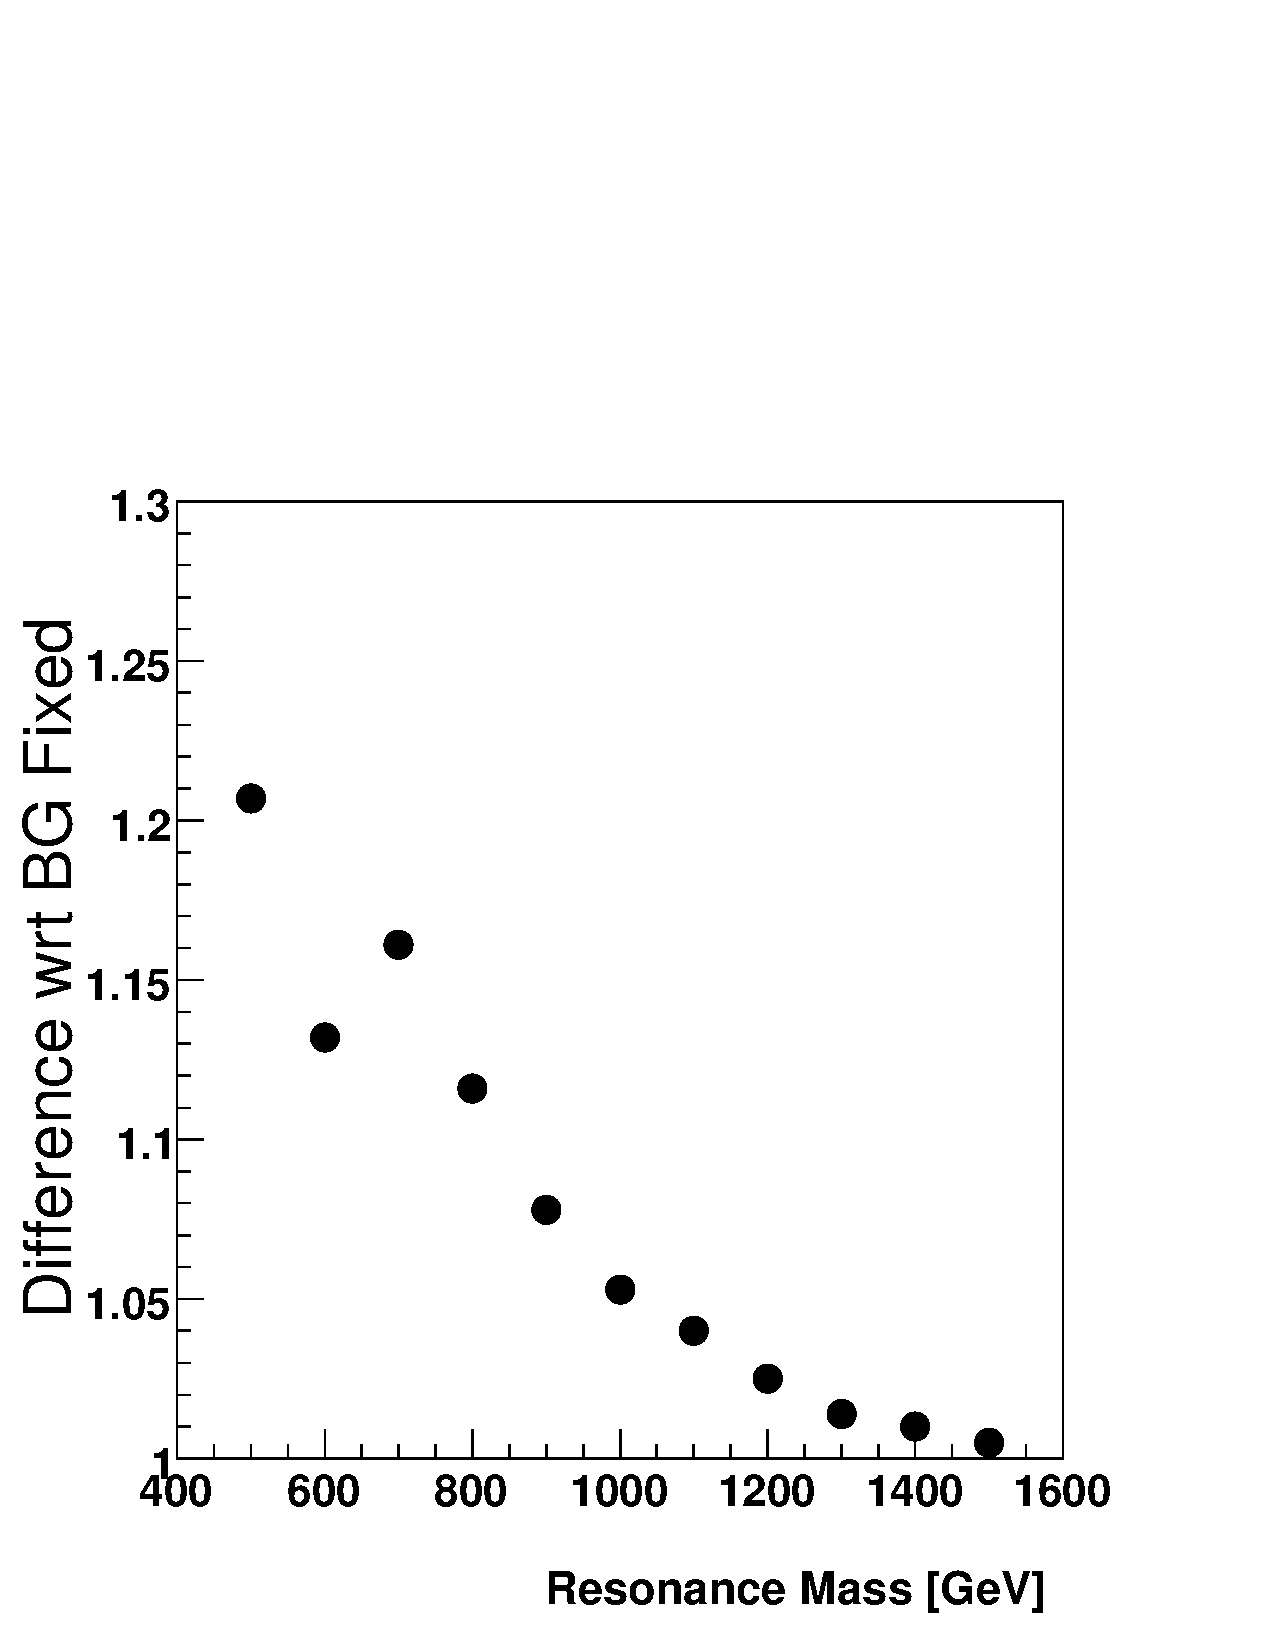
\includegraphics[width=0.7\textwidth]{Figures/DijetMassLimitsProfileLikelihood}
%    \caption{Changes in the 95\% CL upper limits on the $qg$ resonance
%      cross section as a function of resonance masses when the profile
%      likelihood is used, compared to the case in which the background
%      parameters are fixed at the best $Signal+background$ fit. 
%      Analysis done independently with statistics software from CDF (see text).}
%    \label{LimitsProfileLikelihood}
%  \end{center}
%\end{figure}




\begin{table}[htbH]
\centering
\large
\begin{tabular}{|c|c|c|c|}\hline
Mass   &  \multicolumn{3}{c|}{95\% C.L. $\sigma\cdot B$ (pb) Stat. Err. Only}\\
 ($TeV$) &  quark-quark      & quark-gluon  & gluon-gluon\\ \hline
0.5      &  87.5         &  99.0         &  149 \\
0.6      &  129.         &  161.         &  236 \\
0.7      &  64.0         &  93.2         &  192 \\
0.8      &  49.6         &  64.7         &  119  \\
0.9      &  36.8         &  49.4         &  95.1 \\
1.0      &  14.2         &  20.1         &  48.0 \\
1.1      &  11.9         &  14.0         &  23.5 \\
1.2      &  12.0         &  14.2         &  21.9 \\
1.3      &  7.49         &  9.04         &  15.4 \\
1.4      &  4.86         &  6.14         &  11.1 \\
1.5      &  2.68         &  3.56         &  6.96 \\
1.6      &  2.22         &  2.65         &  4.54 \\
1.7      &  2.30         &  2.61         &  4.00 \\
1.8      &  2.18         &  2.47         &  3.68 \\
1.9      &  2.07         &  2.32         &  3.31 \\
2.0      &  2.09         &  2.25         &  3.06 \\
2.1      &  1.96         &  2.15         &  2.93 \\
2.2      &  1.75         &  1.96         &  2.66 \\
2.3      &  1.58         &  1.77         &  2.40 \\
2.4      &  1.49         &  1.64         &  2.16 \\
2.5      &  1.39         &  1.55         &  2.05 \\
2.6      &  1.33         &  1.46         &  1.89 \\
\hline
\end{tabular}
\label{tabStatLimit}
\caption{As a function of resonance mass we list our 95\% C.L. upper limit on
cross section times branching ratio for narrow resonances originating from o
quark-quark, quark-gluon and gluon-gluon pairs of partons, 
including statistical errors only.}
\end{table}


\clearpage
